\documentclass{standalone}
\usepackage{tikz}
\usetikzlibrary{positioning}
\usepackage{calc}

\begin{document}

   \begin{minipage}[c]{0.6cm}
      $f= $
   \end{minipage}
\begin{minipage}[c]{2.5cm}
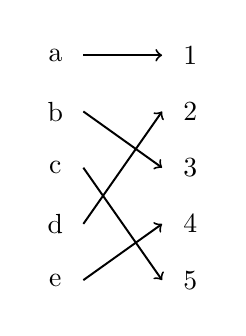
\begin{tikzpicture}[
element/.style={circle, thin, minimum size=7mm},
arrow/.style={->, line width=0.25mm},
]

\node[element] (na) {a};
\node[element] (nb) [below=0cm of na] {b};
\node[element] (nc) [below=0cm of nb] {c};
\node[element] (nd) [below=0cm of nc] {d};
\node[element] (ne) [below=0cm of nd] {e};

\node[element] (n1) [right= of na] {1};
\node[element] (n2) [right= of nb] {2};
\node[element] (n3) [right= of nc] {3};
\node[element] (n4) [right= of nd] {4};
\node[element] (n5) [right= of ne] {5};

\draw[arrow] (na.east) -- (n1.west);
\draw[arrow] (nb.east) -- (n3.west);
\draw[arrow] (nc.east) -- (n5.west);
\draw[arrow] (nd.east) -- (n2.west);
\draw[arrow] (ne.east) -- (n4.west);

\end{tikzpicture}
\end{minipage}

\quad

   \begin{minipage}[c]{0.6cm}
      $g= $
   \end{minipage}

\begin{minipage}[c]{2.5cm}
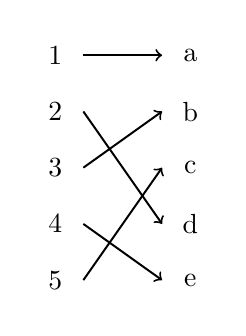
\begin{tikzpicture}[
element/.style={circle, thin, minimum size=7mm},
arrow/.style={->, line width=0.25mm},
]

\node[element] (n1) {1};
\node[element] (n2) [below=0cm of n1] {2};
\node[element] (n3) [below=0cm of n2] {3};
\node[element] (n4) [below=0cm of n3] {4};
\node[element] (n5) [below=0cm of n4] {5};

\node[element] (na) [right= of n1] {a};
\node[element] (nb) [right= of n2] {b};
\node[element] (nc) [right= of n3] {c};
\node[element] (nd) [right= of n4] {d};
\node[element] (ne) [right= of n5] {e};

\draw[arrow] (n1.east) -- (na.west);
\draw[arrow] (n2.east) -- (nd.west);
\draw[arrow] (n3.east) -- (nb.west);
\draw[arrow] (n4.east) -- (ne.west);
\draw[arrow] (n5.east) -- (nc.west);

\end{tikzpicture}
\end{minipage}

\end{document}